\documentclass{exam}

\usepackage{units} 
\usepackage[fleqn]{amsmath}
\usepackage{float}
\usepackage{mdwlist}
\usepackage{booktabs}
\usepackage{caption}
\usepackage{fullpage}
\usepackage{enumerate}
\usepackage{graphicx}

\usepackage{2in1, lscape} 

\everymath{\displaystyle}

\author{}
\title{Statistics \\ Week Four}
\date{\today}

\begin{document}

\maketitle
\tableofcontents

  \section{Homework}

  \begin{description*}
    \item[30]
    \item[32] I didn't mean to assign such a tedious problem.  My bad.
  \end{description*}

  \section{NFL}

  \subsection{Passing Attempts vs. Yards}

  \begin{figure}[H]
    \centering
    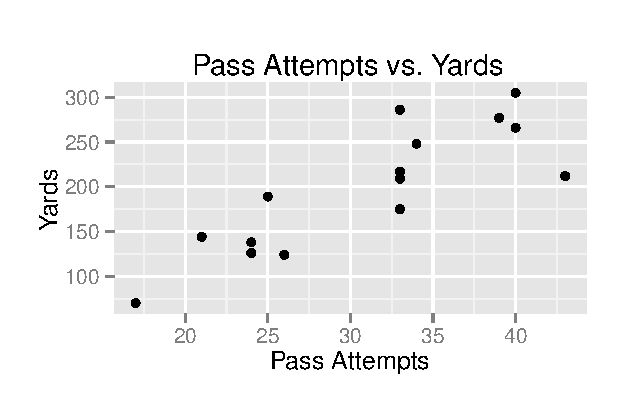
\includegraphics{figures/nfl/passing_attempts_vs_yds.eps}
    \caption{Passing attempts vs. yards}
  \end{figure}

  correlation coefficient: 0.7225

  \subsection{Turnover Differential}

  \begin{figure}[H]
    \centering
    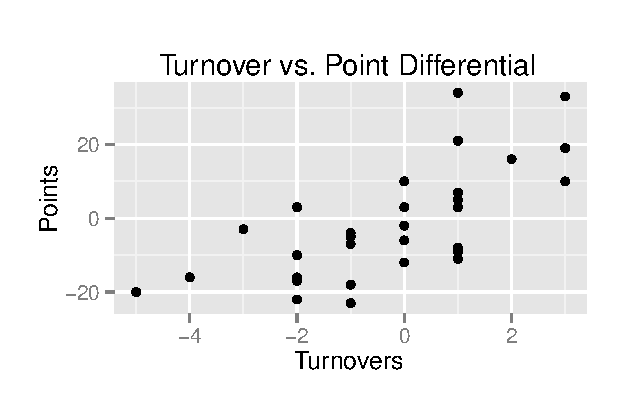
\includegraphics{figures/nfl/to_vs_pts.eps}
    \caption{Turnovers vs. Points}
  \end{figure}

  correlation coefficient: 0.5808
\end{document}

